\documentclass[letterpaper,twocolumn,10pt]{article}
\usepackage{usenix,epsfig,endnotes}
\usepackage{ucs}
\usepackage{url}
\usepackage[T1]{fontenc}
\usepackage[utf8x]{inputenc}

\begin{document}
\date{\today}

\title{\Large \bf SETI@EPFL - a new approach to distributed volunteer computing}
\author{
{\rm Laurențiu Dascălu}\\
{\small \textit{laurentiu.dascalu at epfl.ch}}
\and
{\rm Octavian Ganea}\\
{\small \textit{octavian-eugen.ganea at epfl.ch}}
\and
{\rm Cristian Tălău}\\
{\small \textit{cristian.talau at epfl.ch}}
}

\maketitle

% Use the following at camera-ready time to suppress page numbers.
% Comment it out when you first submit the paper for review.
\thispagestyle{empty}

\subsection*{Abstract}

In this project we present SETI@EPFL a new software platform for volunteer
computing, which leverages the recent progress that has been done in
JavaScript\cite{javascript} execution inside the browsers to provide security,
portability and ease of use.
 
We describe different design decisions that the designer of such a platform
needs to make. We also propose a computation model and the system architecture
that can be used by the developers to build and deploy their computationally 
intensive distributed applications. We also evaluate our system for different 
types of projects.

\section{Introduction}

Volunteer computing is a type of distributed computing in which the owner of
the computers make them available for the use of one or more, usually scientific
projects. Its primary goal is to give to the academic community the computing
power they need in order to make scientific progress at a very little cost. 

Nowadays, there are a lot of projects of this kind, the most popular ones being
SETI@HOME, in which radio telescope data is analyzed in order to find
extraterrestrial intelligence. Another popular project is {\it Great Internet 
Mersenne Prime Search} which found thirteen Mersene prime numbers, eleven of
which were the largest known prime number at their discovery time. Most of the 
current volunteer computing projects use a software platform called BOINC
\cite{boinc} which provides the deployment infrastructure. 

In section \ref{design} we will describe the challenges that occur in
implementing a volunteer computing platform and the solutions given by the state
of the art implementation. Section \ref{seti_epfl} describes SETI@EPFL,
its programming model and architecture. The optimizations and features of our 
system are explained in section \ref{optimizations}. The evaluation and
conclusions are presented in the sections \ref{eval} and \ref{conclusions}.

\section{Challenges in volunteer computing} \label{design}

In general, a volunteer computing project is formed by a small number of
private computers and a huge number of volunteer computers over the Internet.
The volunteer computers are given some code and some data, they feed the data to
the code and submit the results back to the server which aggregates the results.

The ratio between private and volunteer computers is typically one to tens of
thousands, so the time to completion depends heavily on the number of
volunteers. One primary step in gathering more participants to a project is the
{\it ease of setup} that the users need to make. The currently used setup
procedure is to create an account on the project owner's site for identification
purposes and download some executable which is responsible with the
communication with the server. This setup constitutes a barrier for a lots
users that want to contribute.

The code that the volunteers download from the server is usually a binary
executable file. This raises some {\it security and privacy} concerns from the
participant which has to trust that the executable is not malicious. This issue
also contributes to the decrease in the number of volunteers.

From the developer point of view, one challenge is that of {\it portability}:
writing code running on a large heterogeneous set of computers. This creates a 
trade-off between the  development effort and the number of participants that are
able to take part in the project. The solution commonly taken is to have binary
files for major architectures.

Another hard task for the developer is to write the computation in such a way
that it is {\it suitable for volunteer computing}. This means that the computation 
can be split in multiple independent parts that can be easily aggregated, and
that the number of operations per byte is very high so that computation time
pays off for the time needed to keep server busy sending data to the
participant. In SETI@HOME project, the data sent to one participant is less
than 0.5MB and keeps it busy for two days.

The goal of a platform for distributed computing is to {\it provide
infrastructure} to help developer with common tasks as load balancing,
fault tolerance, avoiding client overloading, detecting malicious users, etc.
While good at most infrastructure tasks, BOINC does not provide fault tolerance.

\section{SETI@EPFL} \label{seti_epfl}
\subsection{Proposed solutions}

Our platform, SETI@EPFL, tries to enable volunteer computing for any
Internet user idling on some websites. As just in August 2011, people spent 
41.1 billion minutes on Facebook, we believe that these users offer a great
potential for volunteer computing. 

In order to make it easy to everyone to participate, we don't require clients to
install any client software on their machine - the code that is sent to them is
JavaScript code that runs inside the browser transparently. If the JavaScript
code is embedded in the Facebook page (within a Facebook Application), we can
also use the existing account of the user, making the setup even easier. 

From the security and privacy point of view, the participants are not exposed to
any additional risks than by just visiting a normal website. This is ensured by
the limited access to user computer that is provided by the browser's sandboxing
mechanism.

Another feature that comes for free by the use of JavaScript is portability:
virtually every computer with Internet access has a browser capable of executing
JavaScript code. Even though there are some browser incompatibilities,
computational intensive code is much likely not to depend on them, and our
system provides support for this issue anyway. 

Even if it is very appealing for the participants, the developers are not used
to write distributed programs in JavaScript. To this end, our platform uses
Google Web Toolkit\cite{gwt}, a Java\cite{jvm} to JavaScript compiler, to let
the developers use their favorite programming language.

Our server part is very similar with the one used by BOINC, except that we
checkpoint asynchronously the results using HBase which is run by the primary
server and several backup servers, providing fault tolerance in this way.

One of the problems with this approach may seem to be performance, since
dynamic languages as JavaScript are know to have poor performance. However with
the recent developments in virtual machines and JIT this may not to be the
case any more. However, we expect that the gain in the number of user is
much larger than the slowdown imposed by the language. 

\subsection{Programming model}

Our programming model is based on MapReduce as it closely matches the kind of
tasks that use volunteer computing - tasks which can be split in multiple
independent sub-computations whose results can be easily aggregated together.
Since Hadoop is a popular framework for writing distributed applications, we
expect users to be familiar with this model and to be able to easily port their
existing Hadoop applications to this volunteer computing setting. 

The developer has to submit add three Java classes: 
\begin{itemize}
  \item {\bf MapWorker} - which is compiled to JavaScript with Google Web
  Toolkit and sent to the participants as requested
  {\tt \small \begin{verbatim}
interface IMapWorker<K1 , V1 , K2 , V2> {
  void map(K1 key, V1 value, 
   IOutputCollector<Pair<K2, V2>> output);
} \end{verbatim}}

  \item {\bf ReduceWorker} - which is usually executed on the server, since most
  of the time it is lightweight in terms of computation and provides high security
  risks since it can fake the results given by a large number of participants;
  it can also be sent to clients for execution  
  {\tt \small \begin{verbatim}
interface IReduceWorker<K , V> {
  void reduce(K key, SVector<V> values, 
   IOutputCollector<V> output);
}\end{verbatim}}

  \item {\bf InputGenerator} - which is run on the server and is responsible for
  generating the key-value pairs for the map task. It is dynamically loaded
  on the server as a request from some user comes. A project can implement
  fault-tolerance by implementing the {\tt \small checkpoint} and {\tt
  \small restore} methods.
{\tt \small \begin{verbatim} interface IInputGenerator <K, V> { 
  boolean hasNextTask(); 
  Task<K, V> nextTask();
  boolean executeReduceOnServer();
  void checkpoint(HBaseWrapper db);
  void restore(HBaseWrapper db); 
}\end{verbatim}}

\end{itemize} 

\subsection{Architecture}

\begin{figure*}[!ht]
\begin{center}
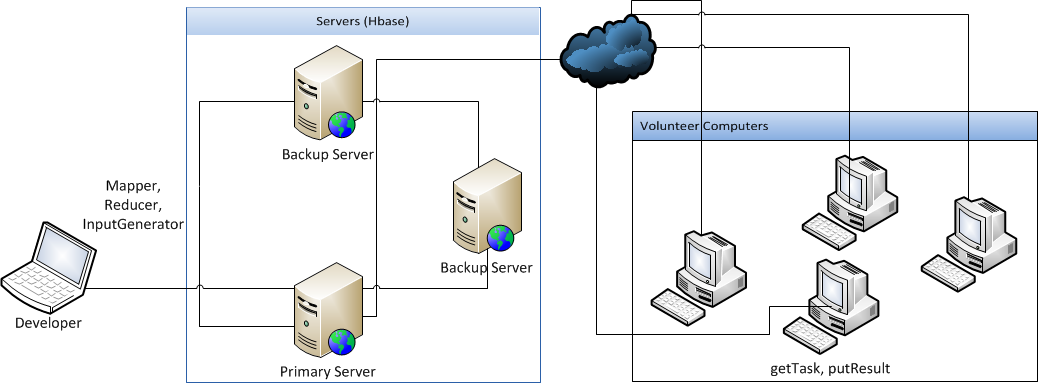
\includegraphics[width=400px]{../imgs/architecture.png}
\end{center}
\caption{System architecture}
\label{fig:architecture}
\end{figure*}

The architecture of our system is presented in Figure~\ref{fig:architecture}.
The developer uploads the source code of the three Java classes and they are
compiled either to Java bytecode, or to JavaScript.

In order to contribute to some project, clients choose the project from a list,
and the corresponding JavaScript code is loaded inside an {\small \tt iframe}.
The code starts to request tasks from the server using an RPC mechanism
implemented over AJAX, execute them and submit the results back. The entire
process is transparent to the user browsing the website.

On the server side, we used servlets to communicate with the client. The state
of the server is checkpointed asynchronously in a HBase instance running on
possibly many computers. Notice that since map operations are idempotent, we 
want only to store as many operations as possible in order to have their results
available after a crash when a backup server takes over. This asynchronous
writing is essential to keep the server responsive. 

We also use a thread pool to execute reduce operations which can also be spread
among the backup servers which are less loaded than the one which is actually
serving the clients.

\section{Optimizations}
\label{optimizations}

We started with optimizing the control flow cost in the Map Reduce model, by
allowing the users to specify where the \textit{reduce} operation should be
done: on the client (JavaScript) or on the server (Java). There are certain
situations where the cost of data transfer is comparable to the reduce operation
(e.g. merge multiple chucks of an image in a bigger image), thus a reduce on
server is preferable over a reduce on client.

The tasks execution is expensive and we decided to analyze the
\textit{performance counters} of a task and mark it as \textit{unsolved} if it
wasn't solved in less than a \textit{timeout} threshold. If multiple clients are
available to work, the system tries to do \textit{speculative execution} (e.g.
two or more clients are executing the same task).

Security is an important issue when talking about distributed systems and
SETI@EPFL has to to deal with poisoned users that submit wrong results. Ideally,
the system has to be able to defend against Byzantine failures\cite{byzantine}.
SETI@EPFL minimizes the time spent on checking if a client is faulty, by
comparing the result only for the tasks that were executed on multiple clients.
Using only this, we will not be able to catch a faulty client that tries to
behave like a normal client, and we introduced the \textit{discovery tasks} that
are special tasks for which the server knows the answer (e.g. how many prime
numbers are within a given interval); if the client is giving a wrong answer,
then it's poisoned and the server should avoid sending tasks to it. This
approach works because it is impossible for the client to distinguish between a
discovery task and a task belonging to a project.

SETI@EPFL optimizes the clients' resources usage by feeding them with work as
soon as they are available. In order to implement \textit{overloading
avoidance}, we can avoid blocking the user's webpage by using {\it web
worker} threads from HTML5, but at the moment the support for them in GWT is in
development. In order to estimate memory consumption we can modify the GWT 
compiler to maintain some counter on object creation. If the task does not obey
the user imposed limits we can kill the worker thread.

\section{Evaluation}
\label{eval}

We evaluated our approach on two examples suitable for the Map-Reduce
programming model: the Mandelbrot\cite{mandelbrot} fractal and the SAT\cite{sat}
problem. Our results include information about the speedup under various
\textit{environment settings} (e.g. different browsers: Internet Explorer, Google
Chrome) and clients' \textit{faultiness} (e.g. a subset of clients is poisoned
and not answering at all). We were interested in server's load during
experiments, and we present graphics for the evolution of CPU, memory and
network consumption.

\subsection{Mandelbrot fractal}

The Mandelbrot fractal problem consists in computing the set of values of $c$ in
the complex plane for which the orbit of 0 under iteration of the complex
quadratic polynomial $z_{n+1} = z_{n}^2 + c$ remains bounded. Each
\textit{Mapper} deals with a subset of values of $c$, which is actually a part
of the image. The \textit{Reducer} simply builds the output image from images
processed by the \textit{Mappers}.

\begin{table}
\begin{center}
  \begin{tabular}{| c | c |}
    \hline
      \textit{Machines \#} & \textit{Execution time} \\
    \hline
      Serial & 72s \\
    \hline
      1 & 33s \\
    \hline
      3 & 12s \\
    \hline
  \end{tabular}
  \label{tab:mandelbrot1024}
  \caption{Mandelbrot 1024x1024}
\end{center}
\end{table}

\begin{table}
\begin{center}
  \begin{tabular}{| c | c |}
    \hline
      \textit{Machines \#} & \textit{Execution time} \\
    \hline
      Serial & 1175s \\
    \hline
      2 & 81s \\
    \hline
      4 & 51s \\
    \hline
      14 & 30s \\
    \hline
  \end{tabular}
  \label{tab:mandelbrot4096}
  \caption{Mandelbrot 4096x4096}
\end{center}
\end{table}

We present the results for the Mandelbrot fractal problem in the tables
\ref{tab:mandelbrot1024} and \ref{tab:mandelbrot4096}. An interesting result is
that the reference implementation, written in Java, takes more than the compiled
JavaScript version; 72 seconds versus 33 seconds. In the end, both programs are
eventually just in time compiled to native code that runs the innermost loop,
and since we are not using any of its dynamic features, there is nothing
unexpected to have the JavaScript faster.

\begin{figure}[!ht]
\begin{center}
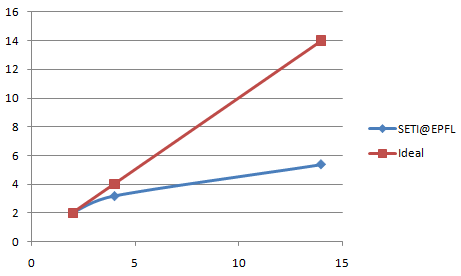
\includegraphics[width=220px]{../imgs/mandelbrot.png}
\end{center}
\caption{Mandelbrot speedup}
\label{fig:mandelbrotSU}
\end{figure}

\begin{figure}[!ht]
\begin{center}
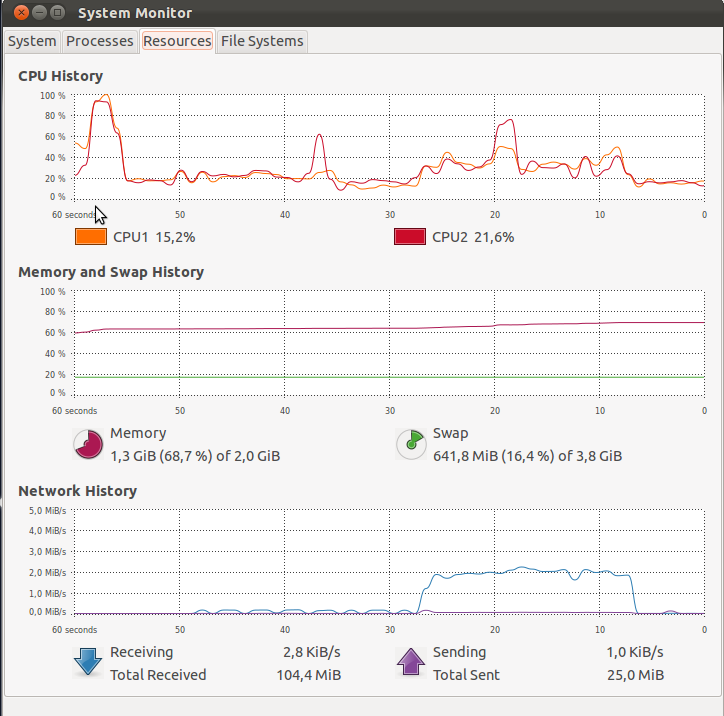
\includegraphics[width=220px]{../imgs/ru-mandelbrot.png}
\end{center}
\caption{Mandelbrot resource utilization}
\label{fig:mandelbrotRU}
\end{figure}

In the figures \ref{fig:mandelbrotSU} and \ref{fig:mandelbrotRU}, we present
the speedup graphics and the resources utilization over time. From these results
we can conclude that the server is on a high consumption of CPU, memory or
network bandwidth. In the network history chart we can see that the server is
active when it has to send tasks for working clients.

\subsection{Boolean satisfiability problem}

The boolean satisfiability problem, abbreviated SAT, is the problem of
determining if the variables of a given boolean formula can be assigned in such
a way as to make the formula evaluate to \textit{true}.

In this example, the input generator assigns some values to $K$ boolean
variables, thus creating a number of $2^K$ \textit{map} tasks. Each
\textit{Mapper} receives some already assigned values and exhaustively searches
for the rest of the variables; it ends exploring $2^{N - K}$ states, where $N$
is the number of boolean variables. The \textit{Reducer} is trivial and simply
collects the valid results from \textit{Mappers}.

\begin{table}
\begin{center}
  \begin{tabular}{| c | c | c |}
    \hline
      \textit{Machines \#} & \textit{Execution time} & \textit{Observations} \\
    \hline
      4 & 461s & {\small Internet Explorer (IE)} \\
    \hline
      4 & 340s & {\small Google Chrome (GC)} \\
    \hline
      8 & 216s & {\small 4 IE, 4 GC} \\
    \hline
      8 & 157s & {\small 8 GC} \\
    \hline
      14 & 73s & \\
    \hline
      14 & 157s & {\small 5 clients closed} \\
    \hline
  \end{tabular}
  \label{tab:sat25}
  \caption{SAT 25 variables}
\end{center}
\end{table}

We present the results for the SAT problem in the table \ref{tab:sat25}. We
tested under various user's configurations (e.g. Internet Explorer and Google
Chrome) and clients' commitments (e.g. some clients are leaving the system
after solving half of the map tasks). Another interesting result is that we
eventually \textit{outperformed} the serial Java version with 14 clients.

\begin{figure}[!ht]
\begin{center}
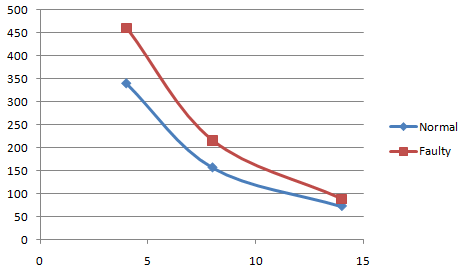
\includegraphics[width=220px]{../imgs/sat.png}
\end{center}
\caption{SAT execution times}
\label{fig:sat}
\end{figure}

In the figure \ref{fig:sat} we present the execution time against the number of
clients. We did a comparative analysis between a \textit{normal} execution, when
all the clients are using Google Chrome and stay until the project is resolved,
and a \textit{faulty} execution, when some clients are using Internet Explorer
and quit after solving a number of tasks.

\section{Conclusions}
\label{conclusions}

In conclusion, we showed an approach of how the \textit{distributed volunteer
computing} (SETI@HOME) can be extended to be more \textit{user-friendly}. We
are using JavaScript to perform computation, which requires just an Internet
browser. Developers don't have to write JavaScript code, as we provide a web
interface where they can submit the Java source code for the project, and
eventually we generate JavaScript code using the Google Web Toolkit.

Our system offers \textit{high security} guarantees for clients' computers,
cause of the limitations of the JavaScript programming language. We evaluated the system and
proved its feasibility. In the context of the Mandelbrot example, the generated
JavaScript code executed on one client outperformed the serial Java code, while
in the context of the SAT problem, we outperformed the serial code with 14
clients; if other clients would have joined the system, then we would have
obtained a lower execution time.

\section{Acknowledgments}

We would like to thank prof. Dejan Kostic for his guidance and teaching
abilities, as part of the Advanced Computer Networks and Distributed Systems,
EPFL, Switzerland, without whom this document would not exist.

\begin{thebibliography}{99}

\bibitem{javascript}
  \url{http://en.wikipedia.org/wiki/JavaScript}

\bibitem{gwt}
  \url{http://code.google.com/intl/ro/webtoolkit/}
  
\bibitem{jvm}
  \url{http://en.wikipedia.org/wiki/Java_Virtual_Machine}

\bibitem{mapreduce}
  MapReduce \url{http://en.wikipedia.org/wiki/MapReduce}

\bibitem{byzantine}
  \url{http://en.wikipedia.org/wiki/Byzantine_fault_tolerance}

\bibitem{mandelbrot}  
  \url{http://en.wikipedia.org/wiki/Mandelbrot_set}

\bibitem{sat}
  \url{http://en.wikipedia.org/wiki/Boolean_satisfiability_problem}
  
\bibitem{boinc}
  \url{http://boinc.berkeley.edu/}

% http://facebook.com
% http://twitter.com
% http://boinc.berkeley.edu/
% http://setiathome.berkeley.edu/
% http://lhcathome.web.cern.ch/LHCathome/
% http://milkyway.cs.rpi.edu/milkyway/
\end{thebibliography}

\end{document}
